\subsection{Robot}
\label{sub:robots}
Gli agenti che modellano il comportamento dei robot sono, di fatto, la componenete principale di tutto il sistema.
Sono i robot, e loro soltanto, a potersi muovere all'interno del territorio cercando i feriti e costruendo, nel mentre, la rete \textit{mesh} per la comunicazione. 
Nonostante abbiano un ruolo così fondamentale, questi agenti sono a tutti gli effetti dei \textit{reflexive agent with internal state} facendo riferimento alla classificazione proposta da Russell e Norvig \cite{russell2016}, il cui comportamento viene descritto di seguito.
È bene esplicitare, prima di proseguire, qual è lo stato interno dell'agente descritto: in questo caso, lo stato interno è dato da un insieme di variabili, in particolare:
\begin{itemize}
	\item \texttt{target\_cell}, ovvero la cella di frontiera a cui il robot è diretto;
	\item \texttt{target\_path} è il cammino minimo che l'agente deve seguire per raggiungere la cella obiettivo dalla posizione attuale;
	\item \texttt{status} serve per indicare se il robot sta esplorando una cella, si sta muovendo, sta scegliendo la prossima cella obiettivo (o sta aspettando che nuove celle si aggiungano alla frontiera) oppure che si è guastato.
\end{itemize}
Per alleggerire la lettura del diagramma di flusso sottostante, e per comodità di descrizione dell'agente, la casistica del fallimento di un robot verrà descritta di seguito separatamente.
Inoltre, come già detto nella Sezione \ref{sec:environment}, questi agenti presentano un insieme di altre variabili che ne descrivono delle caratteristiche o che vengono sfruttate dall'agente per effettuare delle scelte a livello “microscopico” (\textit{e.g.}, quale cella scegliere come obiettivo); a queste si aggiungono tre ulteriori variaibli di interesse: la posizione in cui si trova l'agente, quella precedente e l'utilità della cella scelta come obiettivo prima che venisse modificata (variabile utilizzata per la gestione dei fallimenti dei robot).
Infine, a livello programmativo, sono presenti un insieme di variaibli atte a simulare il tempo che il robot trascorre per spostarsi da una posizione ad un'altra, per esplorare una cella o per il rilascio e la messa in funzione di un ripetitore. 

Durante la sua vita\margin{Comportamento dell'agente}, l'agente valuta il suo stato interno e se sta mantenendo una connessione con la rete \textit{mesh} oppure no; in base a queste due condizioni prende delle decisioni “macroscopiche” su quali azioni effettuare (\textit{e.g.}, decide di rilasciare un ripetitore \textit{wi-fi} oppure di continuare a muoversi verso l'obiettivo), come mostrato in Figura \ref{fig:robotworkflow}.
È importante far notare che il processo decisionale non avviene ad ogni \textit{step} della simulazione (cioè ad ogni secondo d'orologio), ma solo quando lo stato interno del robot subisce delle modifiche.
\begin{figure}
	\centering
	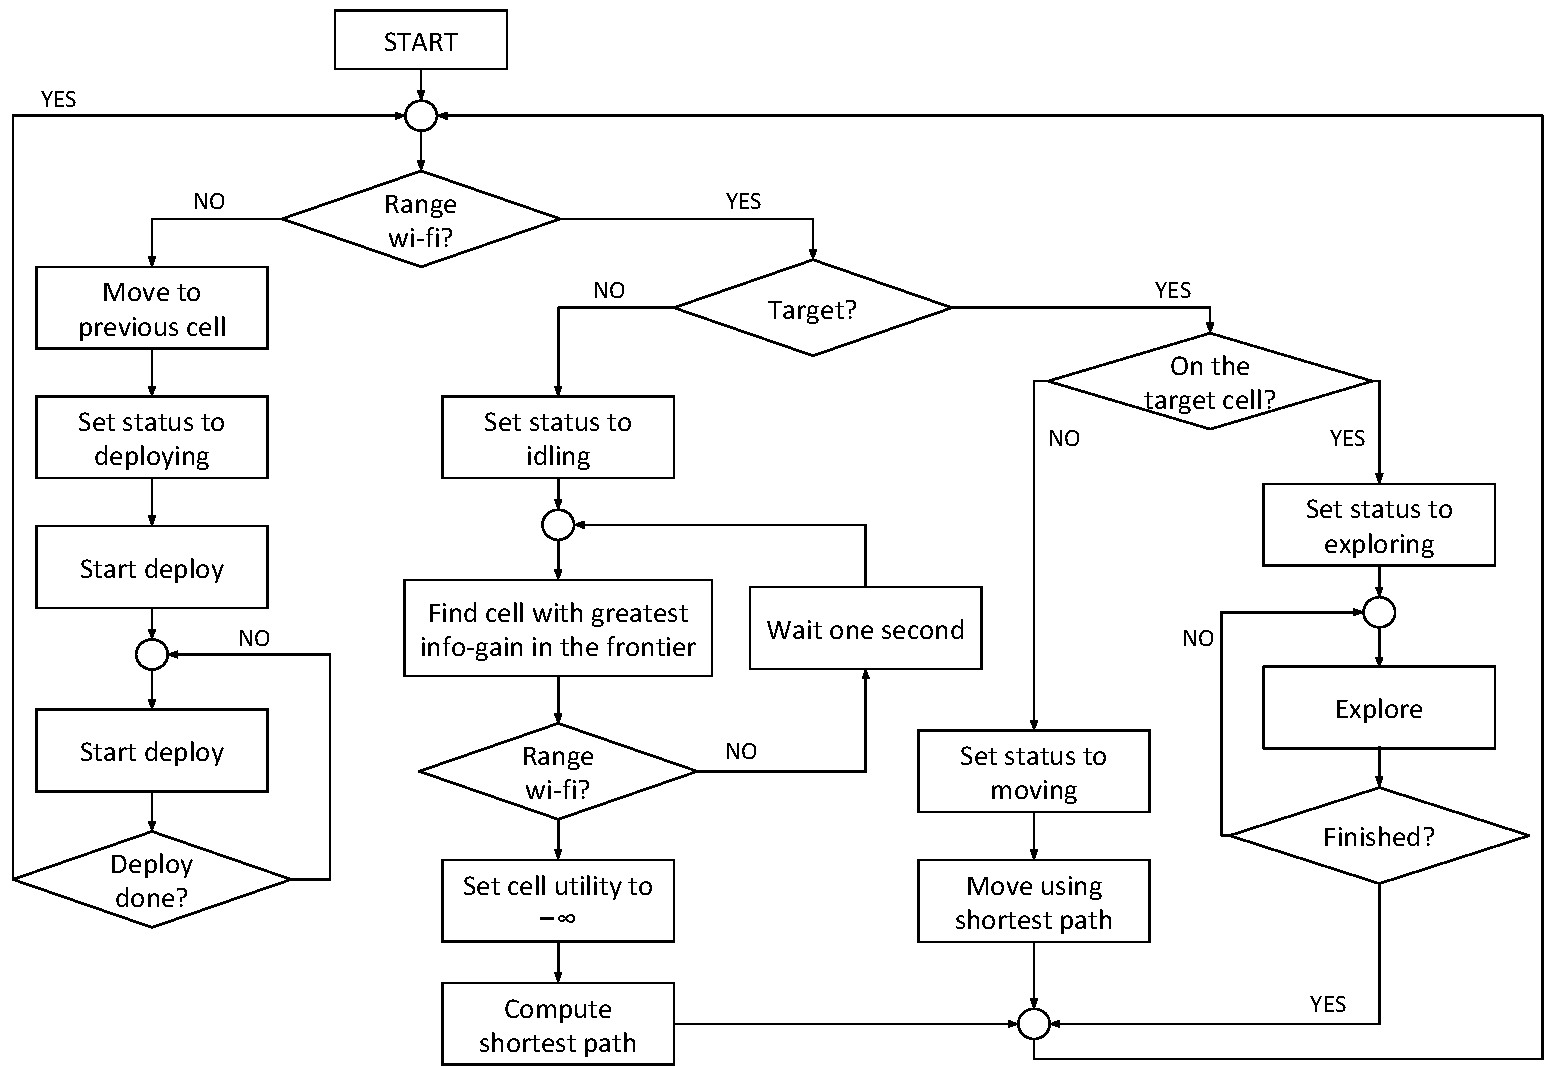
\includegraphics[width=1.0\linewidth]{images/Robot_workflow}
	\caption{Figura che rappresenta il processo decisionale che l'agente robot effettua quando deve stabilire la sua prossima azione. Tale processo si basa sullo stato interno del robot e sulla presenza (o assenza) di connessione con la rete \textit{mesh}; si noti che quello appena descritto non avviene ad ogni step della simulazione, ma solo quando lo stato interno dell'agente subisce dei cambiamenti.}
	\label{fig:robotworkflow}
\end{figure}
Per prima cosa, il robot valuta se è ancora all'interno della copertura \textit{wi-fi} in quanto, per come è stato definito il metodo di comunicazione e coordinamento dei robot, risulta fondamentale che siano sempre in grado di comunicare tra loro.
Tale controllo risulta essere necessario ogni volta che il robot si sposta di una cella, perché è l'unico caso in cui si suppone che l'agente possa perdere la connessione uscendo dall'area coperta; per comodità e “pulizia” algoritmica viene anche effettuato nel caso in cui il robot abbia terminato l'esplorazione di una cella.
Quando il robot, muovendosi, perde la connessione alla rete \textit{wi-fi}, se ne accorge e allo \textit{step} successivo rientra immediatamente nella zona coperta (\textit{i.e.}, la posizione precedente), iniziando poi il processo di rilascio del \textit{bean}: aggiorna il suo stato interno a \textit{deploy}, iniziando poi il processo di rilascio il quale abbiamo supposto impieghi circa 15 secondi (\textit{i.e.}, 15 \textit{step}), poiché il rilascio del ripetitore deve essere effettuato in un luogo e in modo sicuro.\\
Altrimenti, se il robot è in una zona coperta, la sua decisione viene determinata dal possedimento o meno di una cella \textit{target}.
In particolare, se non possiede una cella obiettivo, deve sceglierne una: per prima cosa, si mette in stato di \textit{idling}, ovvero lo stato indicante che il robot è fermo per calcolare il suo prossimo obiettivo (oppure, in casi limite, che non ha celle tra cui scegliere).
In seguito, deve stabilire la cella “migliore” da esplorare; per far ciò, i robot sfruttano un concetto di \textit{information gain} (o \textit{info-gain}), il quale è uno scalare che indica “quanta informazione può portare l'esplorazione di una cella”, ovvero più tale valore è alto più ad un agente conviene andare ad esplorare tale cella. 
La Formula \ref{math:info-gain} è quella utilizzata dagli agenti per il calcolo dell'\textit{info-gain}, tale valore viene calcolato per ogni cella della frontiera.
\begin{equation}
	\label{math:info-gain}
	\textit{Information gain} = \rho+\mu-\alpha\omega
\end{equation}
In tale formula:
\begin{itemize}
	\item $\rho$ è la priorità della cella che risulta essere pari a zero tranne nei casi in cui la cella sia adiacente ad una cella in cui una vittima sia riuscita a segnalare la sua presenza;
	\item $\mu$ è l'utilità della cella;
	\item $\alpha$ è il parametro, già nominato in precedenza, che indica quanto il costo del percorso per raggiungere la cella d'interesse pesi nella scelta. Più il valore è alto, più il costo influisce in maniera significativa e viceversa, ovvero valorizzando di più l'utilità e la priorità delle celle ma non il costo per raggiungerle;
	\item $\omega$ è il costo, in termini di \textit{step} necessari per raggiungere la cella d'interesse attraverso il percorso più breve. 
\end{itemize}
In sostanza, il robot valuta il \textit{trade-off} tra priorità della cella (presenza di un ferito nelle vicinanze), utilità della cella (assenza di altri agenti robotici nelle vicinanze) e costo per il raggiungimento di tale cella. Tale Formula risulta essere lievemente differente rispetto a quella proposta da \cite{burgard2005}, in quanto prende in considerazione anche la priorità di una cella dovuta alla presenza di una richiesta d'aiuto da parte di un ferito.
Si sottolinea che per il calcolo di $\omega$, per ogni cella della frontiera, viene computato il costo del cammino minimo sfruttando la rappresentazione interna del territorio che posseggono (e condividono) i robot sotto forma di grafo delle celle percepite. Precedentemente al calcolo dell'\textit{info-gain}, vengono computati tutti i cammini minimi (e i loro costi) dalla cella in cui è presente il robot verso tutte le altre celle sfruttando l'algoritmo definito da Dijkstra.
Una volta computato l'\textit{info-gain} per ogni cella di frontiera, l'agente sceglie quella con il valore maggiore; essa diventa così la cella \textit{target} dell'agente.
Se il robot è riuscito ad individuare la sua prossima cella obiettivo, imposta l'utilità di tale cella pari a $-\infty$ in modo che nessun altro agente scelga tale cella, memorizza il cammino minimo da intraprendere e poi \textit{rimuove la cella dalla frontiera}. 
Infine, il robot diminuisce l'utilità di tutte le celle del vicinato di \textit{Moore} della cella bersaglio, disincentivando così gli altri robot a convergere nella medesima area.
Si noti che questa riduzione viene inizialmente eseguita a priori per tutto l'intorno della cella bersaglio, senza sapere se effettivamente tutte celle saranno raggiungibili o visibili dal robot una volta giunto sull'obiettivo. Per questo motivo, una volta che l'agente raggiunge il bersaglio, ripristina l'utilità precedente di quelle celle che non riesce a percepire sfruttando i suoi sensori e che sono fuori dalla sua linea “visiva” (\textit{e.g.}, celle dietro ad un ostacolo/muro), annullando di fatto il malus introdotto durante la selezione del bersaglio. In questo modo, tutte le celle che sarebbero visibili dai sensori del robot, ma che non possono venir percepite per via delle macerie (ovvero le celle con valore di \texttt{explored} pari a $-1$) che ne ostacolano la visione, non subiscono la diminuzione di utilità, e ciò permette ad altri robot di essere maggiormente invogliati ad esplorare queste celle. Questa implementazione permette potenzialmente a due robot di viaggiare paralleli sui due lati di un muro, senza che un robot influenzi negativamente l'utilità delle celle viste dall'altro.
La formula di riduzione dell'utilità utilizzata risulta essere differente rispetto a quella proposta nel principale lavoro di riferimento \cite{burgard2005}, ma il principio alla base risulta lo stesso: più la cella è vicina al robot, più la sua utilità viene diminuita, in modo che gli altri agenti siano meno invogliati a muoversi in quella direzione.
La riduzione dell'utilità è definita dalla Formula \ref{math:utility-red}; la differenza rispetto all'articolo è che la riduzione proposta veniva effettuata mediante una sottrazione, che può portare a valori negativi dell'utilità. Dato che tale proposta non ci ha convinto appieno, si è optato per una soluzione che sfrutta lo stesso principio ma che non porta valori negativi di utilità. 
\begin{equation}
	\label{math:utility-red}
	\mu = \mu\times\gamma\left(\frac{\textbf{d}}{\textbf{r}}\right)
\end{equation}
Come in precedenza, $\mu$ è l'utilità della cella, \textbf{d} è la distanza tra le due celle definita come numero di celle da attraversare per raggiungere la destinazione, siano esse celle sugli assi, diagonali o entrambe; invece, \textbf{r} è il raggio di percezione del robot. 
Questa quantità risulta essere tanto più piccola quanto più ci avviciniamo alla posizione del robot, mentre cresce con il progredire della distanza dal robot. Ciò implica che la riduzione dell'utilità sarà inversamente proporzionale alla distanza della cella dal robot.
Infine, $\gamma$ (valore che varia nell'intervallo $\left[0, 1\right]$) stabilisce, di fatto, quanto l'utilità deve venir effettivamente diminuita per il rapporto tra la distanza e il raggio di percezione. 
Qualitativamente, ci si aspetta che quando $\gamma$ è piccola, l'utilità diminuisce in fretta e quindi i robot tenderanno a mantenersi distanti tra loro; al crescere del parametro i robot potrebbero tendere a rimanere più vicini, poiché vi sarebbero celle con utilità elevata anche nelle vicinanze di altri agenti.
Quindi, ad alcuni robot potrebbe risultare conveniente scegliere delle celle con utilità maggiore ma più distanti, si tenga, comunque, presente il metodo di selezione basato sul concetto di \textit{info-gain} e la Formula \ref{math:info-gain}.
Vi sono poi dei casi in cui è possibile che l'agente non riesca a stabilire il suo prossimo obiettivo in quanto non vi sono celle nella frontiera oppure tutte le celle hanno utilità pari a meno infinito e quindi stanno già venendo esplorate da un altro robot; in questi casi, i robot aspettano un secondo prima di aggiornare la rappresentazione del territorio condivisa e cercando nuovamente una possibile cella.\\
Se invece il robot possiede una destinazione, deve verificare se ha raggiunto la posizione designata: se non vi è ancora arrivato continua a muoversi seguendo il cammino minimo, calcolato in precedenza, e aggiorna la sua ultima posizione e quella attuale.
Si noti che durante il processo di movimento il robot continua a verificare di essere ancora all'interno della copertura del segnale; se ciò non dovesse essere soddisfatto, incomincia la fase di rilascio del ripetitore per poi riprendere a muoversi sfruttando il cammino minimo calcolato in precedenza.
Invece, se l'agente si trova nella cella designata, esso modifica il suo stato e inizia la \textit{routine} di esplorazione.\\
Una volta finita l'esplorazione, tutto il processo appena descritto viene ripetuto da capo.

Fin'ora è stato dato per scontato\margin{Comunicazione tra gli agenti} come i robot comunichino tra loro.
Nonostante la completezza dei meccanismi di comunicazione non sia stata implementata direttamente all'interno del simulatore, poiché è stato considerato un problema che esulasse dagli obiettivi del lavoro, ci teniamo a sottolineare come abbiamo pensato sia realizzabile in linea teorica il meccanismo di comunicazione, e quindi perché sono state utilizzate delle “semplificazioni” programmative a livello di simulatore.
L'idea principale del metodo proposto è che i robot mentre esplorano costruiscono la rete \textit{mesh} che non solo permette ai feriti di segnalare la loro posizione mediante l'utilizzo del GPS, ma permette anche ai robot di comunicare tra loro come con una qualsiasi rete \textit{wi-fi}.
Di conseguenza, per come è stato proposto il meccanismo della rete \textit{mesh} \cite{yarali2009wireless} che richiede la presenza di un ripetitore madre, si è pensato che tale ripetitore (o un pc ad esso collegato) possa tenere in memoria l'insieme delle coordinate GPS che rappresentano la frontiera e la rappresentazione della mappa del territorio che sta venendo esplorato dai robot: una rappresentazione a grafo analoga al \texttt{seen\_graph} descritta nella Sezione \ref{sec:environment}.
In particolare, ogni nodo rappresenta una cella, un'area di 3$\times$3 metri indicata da una coordinata GPS ricadente in tale area; gli archi rappresentano i passaggi possibili da un'area ad un'altra con un peso che indica la difficoltà stimata di attraversamento. Tale peso è stabilito dalla difficoltà della cella indicata dal nodo sorgente dell'arco.
In questo modo, i robot hanno tutte le informazioni necessarie: quali celle sono state viste (i nodi del grafo), la loro difficoltà stimata di attraversamento (il peso degli archi) e quali sono le celle appartenenti alla frontiera.
Poiché è garantito che i robot siano sempre nelle copertura della rete, ogni volta che devono comunicare qualcosa (\textit{i.e.}, la vista effettiva del territorio in nuove coordinate oppure il ritrovamento di un ferito) o prendere una qualche decisione (\textit{i.e.}, la prossima cella obiettivo), prima richiedono la versione aggiornata di tali dati e poi comunicano le eventuali novità scoperte o aggiornano i valori all'interno della rappresentazione del territorio.
Tali comunicazioni, come già detto, sono state rese trasparenti poiché le riteniamo un problema puramente tecnico e di poco costo temporale rispetto alla scala considerata nel lavoro. Di conseguenza, è stata preferita una rappresentazione a livello programmativo di tali dati direttamente nella classe che descrive l'ambiente (come già detto) e quindi direttamente condivisa tra tutti gli agenti.

\todo[inline]{fallimenti parlarne altrove? DP}

\subsection{Ferito}
\label{Ferito}
Questo agente rappresenta una persona ferita che è dispersa nell'area di interesse e necessita di essere individuata e salvata. Si noti che il meccanismo di salvataggio non fa parte di questo simulatore, poiché le metodologie di salvataggio dipendono da fattori esterni che non possono venir considerati complessivamente in un simulatore (\textit{e.g.}, la loro possibilità di muoversi oppure se richiedono un intervento medico sul campo).
Il loro comportamento è stocastico, ma basato su uno stato interno; di conseguenza tali agenti sono stati classificati come \textit{reflexive agent with internal state}, facendo nuovamente riferimento alla classificazione proposta da Russell e Norvig \cite{russell2016}.
L'agente è molto semplice, possiede solo due attributi che lo descrivono: la posizione all'interno della griglia e lo stato interno. Lo stato assume valore 0 nel momento in cui il ferito non è ancora stato trovato da un robot e 1 quando invece è stato individuato.
Il suo comportamento, come detto, dipende dal suo stato interno, in particolare: 
\begin{itemize}
	\item finché tale agente non è stato individuato e la cella in cui si trova non è coperta dal \textit{wi-fi} non fa nulla;
	\item se si trova in una cella coperta e non è ancora stato individuato, ha una probabilità pari a $10^{-3}$ di segnalare la sua presenza collegandosi alla rete \textit{mesh}. Tale probabilità risulta essere bassa perché bisogna considerare che ad ogni \textit{step} (un secondo di tempo d'orologio) della simulazione un ferito può segnalare la sua presenza ed inoltre non tutte le persone potrebbero aver accesso ad un telefono in una situazione critica;
	\item se è stato individuato da un robot o ha già segnalato la sua presenza, non fa altro che aspettare.
\end{itemize}

\margin{Metodologie di prioritizzazione}
L'ambiente permette inoltre ai feriti non ancora individuati che si ritrovano coperti dalla rete \textit{mesh} creata dai robot di collegarsi ad essa e segnalare così la loro presenza. Per fare in modo che i robot siano invogliati ad esplorare in modo prioritario le celle in cui è presente un ferito, alla cella da cui è partita la richiesta di aiuto ed al suo vicinato di ordine uno viene assegnato un valore di utilità diverso da $0$. Un primo metodo di assegnamento di questo valore è un valore fisso, in particolare $1$ per la cella che ha emesso il segnale di aiuto e $1/3$ per il suo vicinato. Questo metodo risulta essere più o meno efficace, generando una convergenza dei robot sul punto più o meno forte in base al valore di $\alpha$ impostato nella simulazione: un valore alto porterà i robot a ignorare le celle, se vi è una cella più vicina o meno difficile da raggiungere, mentre un valore basso porterà tutti i robot a convergere nell'area, considerando marginale il costo per raggiungere la cella. Per ovviare a questo, è stata implementata una seconda strategia di assegnazione dei valori di priorità; in particolare, viene assegnato alla cella in cui si trova il ferito una priorità pari a 
$\alpha \cdot 6 \cdot wifi\_range$. Questo valore rappresenta il massimo costo possibile che un robot dovrà sostenere per raggiungere la cella dal margine del segnale del ripetitore \textit{wifi}. In questo modo vi è la garanzia che, qualora un robot fosse nel raggio del ripetitore, esso avrà una forte attrazione verso questa cella, indipendentemente dal valore di $\alpha$ impostato dalla simulazione. Al fine di evitare fenomeni in cui tutti i robot convergono nell'area, è stato deciso di assegnare un valore di priorità all'intorno della cella contenente il ferito pari a $\alpha \cdot 6$, ovvero andare a eguagliare il massimo costo di spostamento da un cella confinante verso questa cella. Ciò porterà l'eventuale robot che ha esplorato la cella del ferito a prioritirizzare l'esplorazione del suo intorno, ma non richiamerà l'intera flotta di robot ad esplorare un'area ristretta.
